\chapter{Preliminares}

En este capítulo vamos a presentar las herramientas básicas para llevar a cabo el desarrollo del trabajo. Empezaremos recordando conceptos básicos de probabilidad, presentaremos algunos resultados relacionados con las matrices positivas y finalmente daremos un breve repaso a la idea de programación dinámica.

\section{Conceptos básicos de probabilidad}
Comenzamos presentado los elementos necesarios para definir una probabilidad:
\begin{definition}
    Sea $\Omega$ un conjunto arbitrario, diremos que una familia no vacía de subconjuntos de $\Omega$, $\mathcal{A}\subseteq\mathcal{P}(\Omega)$, siendo $\mathcal{P}(\Omega)$ conjunto potencia de $\Omega$, es una $\sigma$-álgebra si:
    \begin{itemize}
        \item Es cerrada para complementarios: $\forall A\in\mathcal{A},\, \Omega\setminus A\in\mathcal{A}.$
        \item Es cerrada para uniones numerables: si $A_{n}\in\mathcal{A}, \,\forall n\in\mathbb{N}  \implies \displaystyle\bigcup_{n\in\mathbb{N}}A_n\in\mathcal{A}.$
    \end{itemize}
\end{definition}

A la dupla $(\Omega,\mathcal{A})$ se le conoce como espacio medible.
\begin{definition}
    Sea $(\Omega,\mathcal{A})$ un espacio medible, $P:\mathcal{A}\longrightarrow [0,1]$ es una probabilidad si:
    \begin{itemize}
        \item $P(A)\geq 0, \, \forall A\in\mathcal{A}.$
        \item $P(\Omega)=1.$
        \item Dada una secuencia $\{A_{n}\}_{n\in\mathbb{N}}\subseteq\mathcal{A}$ con $A_i\centernot\cap A_j$, $i\neq j$ entonces:
        \[P\left(\bigcup_{n\in\mathbb{N}}A_n\right)=\sum_{n\in\mathbb{N}}P(A_n).\]
    \end{itemize}
\end{definition}
A la terna $(\Omega,\mathcal{A},P)$ se le conoce como espacio probabilístico.
\begin{definition}
    Sea $(\Omega,\mathcal{A},P)$ un espacio probabilístico y $A\in\mathcal{A}$ con $P(A)>0$. Sea $B\in\mathcal{A}$, se define la probabilidad de $B$ condicionada a $A$ como:
    \[P(B|A)=\dfrac{P(B\cap A)}{P(A)}.\]
\end{definition}
Relacionado con esta definición presentamos el siguiente teorema que nos será útil:
\begin{theorem}[Teorema de probabilidad total]
    Sea $(\Omega,\mathcal{A},P)$ un espacio probabilístico y $\{A_{n}\}_{n\in\mathbb{N}}\subseteq\mathcal{A}$ una partición de $\Omega$ con $P(A_n)>0, \,\forall n \in \mathbb{N}$. Sea $B\in\mathcal{A}$, entonces:
    \[P(B)=\sum_{n\in\mathbb{N}}P(A_n)P(B|A_n).\]
\end{theorem}
\begin{proofs*}
    Por ser $\{A_n\}$ una partición de $\Omega$, aplicando la definición de probabilidad condicionada y teniendo en cuenta que $P(A_n)>0$:
    \[P(B)=P\left(\bigcup_{n\in\mathbb{N}}B\cap A_n\right)=\sum_{n\in\mathbb{N}}P(B\cap A_n)
        =\sum_{n\in\mathbb{N}}P(A_n)P(B|A_n).\]\qed
\end{proofs*}

\begin{definition}
 Sea $(\Omega,\mathcal{A},P)$ un espacio probabilístico y $(\Omega',\mathcal{A}')$ un espacio medible. Una función $X:(\Omega,\mathcal{A},P)\longrightarrow(\Omega',\mathcal{A}')$ es una variable aleatoria si:
 \[X^{-1}(B)\in\mathcal{A}, \quad \forall B\in\mathcal{A}'.\]
\end{definition}

\section{Matrices positivas}
Para el estudio de las cadenas de Markov, necesitaremos algunos resultados previos sobre matrices. Por comodidad, usaremos a lo largo de este trabajo la notación fila para representar los vectores. Los contenidos de esta sección se basan principalmente en \cite{Salinelli}.

\begin{definition}
    Sea una matriz $A=[a_{ij}]$, diremos que $A$ es:
    \begin{itemize}
        \item \textbf{no negativa} si $a_{ij}\geq 0,\, \forall i,j$.
        \item \textbf{positiva} si $a_{ij}\geq 0,\, \forall i,j$ y existe $a_{ij}>0$ para al menos un par de índices $i,\,j$.
        \item \textbf{estrictamente positiva} si $a_{ij}> 0,\, \forall i,j$.
    \end{itemize}
\end{definition}

\begin{definition}
    Sea $A=[a_{ij}]$ una matriz cuadrada de dimensión $N$, diremos que $A$ es una \textbf{matriz estocástica} si:
    \[
    \begin{aligned}
    a_{ij}\in[0,1],\quad \forall i,j \in \{1,...,N\},\\
    \sum_{j=1}^N a_{ij}=1, \quad \forall i\in\{1,...,N\}.
    \end{aligned}
    \]
\end{definition}

Una forma de caracterizar las matrices estocásticas es mediante la siguiente proposición:

\begin{proposition}\label{propiedadMatrizEstocástica}
Sea $A$ una matriz cuadrada positiva de dimensión $N\times N$:
\begin{enumerate}
    \item $A$ es estocástica si y solo si $1$ es un valor propio de $A^T$ con vector propio $\mathbf{1}=\begin{pmatrix}1 & 1 & \dots & 1\end{pmatrix}$.
    \item si $A$ es estocástica, entonces para todo valor propio $\lambda$, se cumple que  $\left|\lambda\right|\leq1.$
\end{enumerate}
\end{proposition}

\begin{proofs*}
\
\begin{enumerate}
    \item Es suficiente con observar que la condición de estocasticidad para una matriz positiva $A$ es equivalente a que $\mathbf{1}\cdot A^T=\mathbf{1}$.
    \item Sea $v=(v_1,\dots,v_N)$ un vector propio asociado a $\lambda$ (a izquierda pues estamos usando la notación fila), por ser $A$ positiva y estocástica, se verifica:
    \[
    \begin{aligned}
        \left|\lambda\right|\sum_{j=1}^N\left| v_j\right|&=\sum_{j=1}^N\left|\lambda v_j\right|= \sum_{j=1}^N\left|(vA)_j \right|  =\sum_{j=1}^N\left|\sum_{i=1}^N a_{ij}v_i\right|\\
        &\leq\sum_{j=1}^N\sum_{i=1}^N a_{ij}\left|v_i\right|=\sum_{i=1}^N\left( \sum_{j=1}^N a_{ij} \right) \left|v_i\right|=\sum_{i=1}^N\left|v_i\right|.    
    \end{aligned}
    \]
    Puesto que $\displaystyle\sum_{r=1}^N\left|v_r\right|>0$, tenemos que $\left|\lambda\right|\leq1$.    \qed
\end{enumerate}
\end{proofs*}

\begin{remark*}\label{productoEstocásticos}
De la primera afirmación de la proposición \ref{propiedadMatrizEstocástica}, podemos ver que el producto de matrices estocásticas sigue siendo estocástica. En efecto, si $A$ y $B$ son dos matrices estocásticas entonces $\mathbf{1}\cdot\left(AB\right)^T=\mathbf{1}\cdot B^T\cdot A^T=\mathbf{1}\cdot A^T=\mathbf{1}$.
\end{remark*}

Presentamos a continuación la definición de grafo dirigido y grafo de una matriz no negativa:
\begin{definition}
    Un grafo dirigido $G$ es un par $(V,L)$ donde $V=\{v_1,\dots,v_n\}$ es un conjunto finito de elementos llamados \textbf{nodos} (o \textbf{vértices}) y $L=\{l_1,\dots,l_m\}\subseteq V\times V$ es un conjunto de pares ordenados de dichos nodos llamados \textbf{arcos} (o \textbf{aristas}).
\end{definition}

\begin{definition}
    Sea $G=(V,L)$ un grafo dirigido, un \textbf{camino dirigido} $C$ desde $v_{i_0}$ a $v_{i_p}$ es una secuencia de nodos $C=\{v_{i_0},v_{i_1}, \dots, v_{i_p}\}$ tal que $v_{i_k}\in V$ para todo $k=0,\dots,p$ y $(v_{i_{k-1}}, v_{i_k})\in L$ para todo $k=1,\dots,p$. 
\end{definition}

\begin{definition}
    Sea $G=(V,L)$ un grafo dirigido, diremos que:
    \begin{itemize}
        \item un nodo $v_i\in V$ está \textbf{conectado} con un nodo $v_j\in V$ si existe un camino dirigido de $v_i$ a $v_j$.
        \item un nodo $v_i\in V$ está \textbf{fuertemente conectado} con un nodo $v_j\in V$ si ambos están conectados.
    \end{itemize}
    Un grafo dirigido está \textbf{fuertemente conectado} si sólo tiene un nodo o todos sus nodos están fuertemente conectados entre ellos.
\end{definition}

\begin{definition}
    Sea $A$ una matriz cuadrada no negativa de dimensión $N$, el grafo dirigido asociado a $A$ es de la forma $G_A=(V_A,L_A)$ donde:
    \[V_A=\{1,\dots,N\},\] 
    \[L_A=\{(i,j)\in V_A\times V_A \,|\, a_{ij}>0\}.\]
\end{definition}

\begin{exampleth}
    Dada la matriz:
    \[A=\begin{pmatrix}
        2 & 0 & 1 & 6 \\
        0 & 4 & 2 & 3 \\
        1 & 5 & 0 & 0 \\
        7 & 3 & 1 & 1 
    \end{pmatrix}\]
    Podemos representar su grafo asociado:
    \begin{center}
        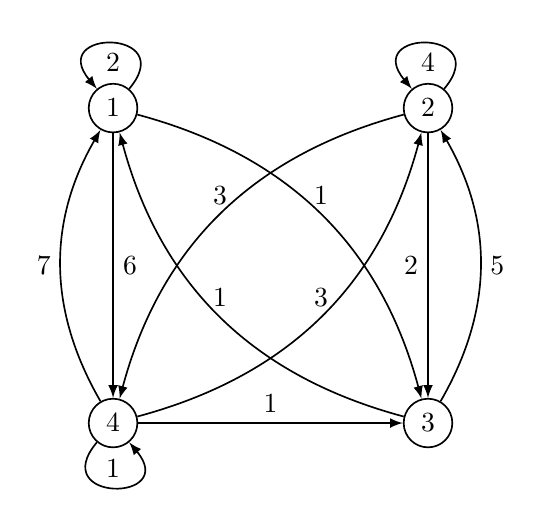
\begin{tikzpicture}[-latex ,auto , node distance =4 cm ,semithick,
        main/.style = {draw, circle}] 
            \node[main] (1) {$1$}; 
            \node[main] (2) [right of=1] {$2$};
            \node[main] (3) [below of=2] {$3$};
            \node[main] (4) [below of=1] {$4$};
            
            \path (1) edge[distance=1cm, out=50, in=130] node {2} (1);
            \draw (1) edge [bend left] node [above] {1} (3);
            \draw (1) edge node {6} (4);

            \path (2) edge[distance=1cm, out=50, in=130] node {4} (2);
            \draw (2) edge node[left] {2} (3);
            \draw (2) edge[bend right] node [above] {3} (4);

            \path (3) edge[bend left] node [above] {1} (1);
            \path (3) edge[bend right] node[right] {5} (2); 

            \path (4) edge[bend left] node {7} (1); 
            \path (4) edge[bend right] node [above] {3} (2);
            \path (4) edge node {1} (3);
            \path (4) edge[distance=1cm, out=230, in=310] node {1} (4);
            
        \end{tikzpicture}
    \end{center}
    El grafo de esta matriz está fuertemente conectado pues desde cualquier nodo podemos encontrar un camino dirigido a cualquiera de los otros nodos, incluido a él mismo.
\end{exampleth}

A continuación presentaremos dos tipos especiales de matrices y algunos resultados relacionados que nos servirán en el siguiente capítulo:
\begin{definition}
Sea $A$ una matriz cuadrada no negativa, se dice que $A$ es \textbf{irreducible} si $G_A$ está fuertemente conectado.
\end{definition}

\begin{theorem} \label{propiedadMatrizIrreducible}
    Sea $A$ una matriz irreducible, entonces:
    \begin{enumerate}
        \item Existe un valor propio positivo y simple  $\lambda_1$ tal que para todo valor propio $\lambda$, se tiene que $\lambda_1\geq\lambda$.
        \item Existe un único vector propio asociado a $\lambda_1$ con todos las componentes estrictamente positivas.
        \item Todos los valores propios con módulo igual a $\lambda_1$ son simples.
    \end{enumerate}
\end{theorem}
\begin{proofs*}
    Véase \cite[Página 263, Teorema 7.13]{Salinelli}.\qed
\end{proofs*}

\begin{definition}
    Sea $A$ una matriz cuadrada positiva, se dice que $A$ es \textbf{primitiva} si existe $k\in\mathbb{N}$ tal que $A^k$ es estrictamente positiva.
\end{definition}

\begin{theorem}[Teorema de Perron-Frobenius] \label{Perron-Frobenius}
    Sea $A$ una matriz primitiva, entonces:
    \begin{enumerate}
        \item $A$ tiene un valor propio $\lambda_1$ real, estrictamente positivo y dominante, esto es:
        \[|\lambda_i|<\lambda_1,\; \forall\lambda_i\in\sigma(A)\setminus \{\lambda_1\}\]
        y $\rho(A)=\lambda_1$.
        \item Se puede tomar un vector propio $v_1$ asociado al valor propio $\lambda_1$ con todas las componentes estrictamente positivas.
    \end{enumerate}
\end{theorem}
\begin{proofs*}
    Véase \cite[Página 202]{Salinelli}.\qed
\end{proofs*}
Como consecuencia de este teorema tenemos el siguiente corolario:
\begin{corollary} \label{colorarioPerron}
    Sea $A$ una matriz primitiva de dimensión $N\times N$, $\lambda_1$ su valor propio real, estrictamente positivo y dominante y $v_1$ un vector propio asociado a $\lambda_1$. Entonces, sea $X_0$ un vector de dimensión $N$ con todas las componentes no negativas y al menos una componente estrictamente positiva:
    \[\underset{n\rightarrow\infty}{lim}\frac{1}{||X_0A^n||_1}X_0A^n=\frac{1}{||v_1||_1}v_1.\]
\end{corollary}
\begin{proofs*}
    Véase \cite[Página 201, Teorema 5.19]{Salinelli}.\qed
\end{proofs*}

\section{Programación dinámica}
A continuación recordaremos brevemente la idea fundamental de la programación dinámica, esta técnica se verá aplicada en los distintos algoritmos que iremos presentando a lo largo de este trabajo. Esta sección se ha basado en contenidos de \cite{algoritmia}.

Cuando encontramos un problema, lo lógico es dividirlo en problemas de menor tamaño siempre que sea posible, resolver dichos subproblemas y combinar las soluciones para resolver el problema original. Puede ocurrir de forma natural que al dividir el problema original obtengamos subproblemas que necesitan para su resolución realizar los mismos cálculos más de una vez. Para evitar repetir las mismas operaciones en varias ocasiones, se puede crear una tabla donde se almacenen los resultados de las operaciones realizadas y que se irá rellenando a medida que se vayan resolviendo los subproblemas. En esta idea simple, es en lo que se apoya la programación dinámica.

No obstante, sólo podemos emplear programación dinámica en aquellos problemas en los que sea aplicable el principio de optimalidad. Este principio afirma que en una sucesión óptima de decisiones u opciones, toda subsucesión debe ser también óptima. Los problemas típicos en los que no es aplicable el principio de optimaliadad son problemas sobre la utilización de recursos limitados. En dichos casos, la combinación de soluciones óptimas de subproblemas puede conllevar a superar el límite de recursos.

Cuando es aplicable el principio de optimalidad a un problema, entonces la solución óptima es una combinación de soluciones óptimas de aquellos subproblemas que sean relevantes para el problema original considerado. Por lo tanto, la programación dinámica resuelve todos los subproblemas, determina los que son realmente relevantes y finalmente combina las soluciones en una solución óptima del problema original.